\chapter{Experimental part: Data cleaning}
\label{chap:clean}
In this chapter, we will present the process of the raw dataset cleaning. As we discussed in previous sections, we extracted raw web features separately for event components (name, date, location, description) and random elements of the page. We aim to construct train dataset with both positive and negative examples for every event component to build binary classifiers. \\

This chapter opens the block of the chapters which cover the Experimental part of the thesis. We will often refer to the Python code which may be found in corresponding Jupyter notebooks. In this chapter, we cover the main stages and present the scheme of the whole cleaning pipeline. Also, we will show how the raw data is melting, meaning after the every step of the cleaning process the amount of data is reducing dramatically. The less significant results will be available in Appendix chapter. The whole process together with the corresponding code you may see in the notebooks with the prefix \textit{Clean}.\\

The process of big dataset cleaning usually is very time-consuming, and in our thesis, it was not an exception. The reason for this in our case is that the dataset is artificial and collected from the Internet by our crawlers. During the collecting stage, we could face problems with the web element availability, encoding, duplicates, missing values and all other natural effects. We separated the whole process into 4 logical components. In the first part we remove the rows which have a visible damage. In the second part we look closer and work individually with the CSS properties since there are more than 200 features and not all of them are relevant for us. In the third part, we work with \textit{frequent domains} which have a lot of similar URL pages. In the last part, we worked with the outliers and logically not-existing values of the features. \\

On the picture \nameref{fig:clean} you main see the main stages of the cleaning process.

\begin{figure}[h]
\begin{center}
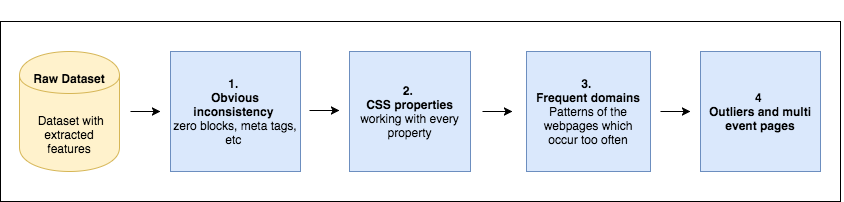
\includegraphics[width=1.0\textwidth]{figures06/clean_workflow1}
\caption{Raw data-cleaning workflow}
\label{fig:clean}
\end{center}
\end{figure}

Let's discuss every part of this scheme.\\

\section*{Obvious inconsistency}

Here we worked with several types of inconsistency:

\begin{itemize}
    \item Duplicates of rows by numerical features.
    \item The 'meta' tag. Developers often set the meta information with semantic schema not in the associated real web element, but rather to an artificial auxiliary tags 'meta'. These artificial tags don't fall into a render tree because they are not visible. That means the data like this is unnecessary because it doesn't contain any visual relevant information we extract. With this filtering, we lost of data.  
    \item Zero block width and height.
    \item Zero X and Y coordinates
    \item Empty URL
\end{itemize}

Corresponding code for this step you may see in the notebook with the prefix \textit{Clean I}.


\section*{CSS properties}
In out Raw dataset we have 288 CSS features from a virtual web browser. To get these properties the browser rendered the page, so we have real post-processing values of CSS fields. Many of properties have prefix \textit{-webkit}. Webkit is a rendering engine used by Safari, Chrome, and other browsers. The \textit{-webkit} prefix on CSS selectors are properties that only this specific engine is intended to process. Due to inconsistency in a browser rendering engines, developers need to set multiple rules for the same thing for all popular browsers, that's the reason why web developers community is hoping this goes away. From our point of view, that means we have a lot of duplicated or almost the same features which don't add new information.\\

Here is a list of steps we made for working with CSS features:

\begin{enumerate}
    \item Remove duplicated columns.
    \item Remove those columns one where the there is a default value is been set for every row in a dataset. For example auto, nonzero, normal, etc. 
    \item Replaced sub-string 'px' in every cell to extract numerical pixel value.
    \item Calculated the proportion of 'NaN' and 'None' values for every column. Then remove those columns we the percentage was greater than 30\%. We saw a big jump from 30\% to 90\% without intermediate values, so it looked like a safe threshold. See \nameref{table:cssnan}
    \item Calculate unique values of CSS properties and removed that one where the value is not a categorical one.   
    \item Then work specifically with the 12 color properties. After we had examined their values, it appears that almost all of them were the same or had default values. So we decided to leave only one main \textit{color} property which has the form \textit{'rgb(number, number, number)'}. We extracted these three values for red, green and blue channels into three new features. 
    \item Extract a font family from the corresponding column into one separate feature.
    \item On this stage we had only 12 CSS properties left. Then we considered categorical features as \textit{display, font\_family, text\_align, tag, display} and made label encoding with the value between 0 and (number of classes - 1) for every feature.
    \item Then we processed two features \textit{font\_weight} and \textit{line\_height}. These two properties had both numerical and categorical values. For example, \textit{font\_weight} has values as 100,200, etc and at the same time 'normal' and 'bold'. We looked at the documentation and replaced the categorical value with the corresponding numerical one. 
\end{enumerate}

The final list of 12 CSS features as follows: \textit{x\_coords, y\_coords, block\_height, block\_width, tag, num\_child, color\_r, color\_g, color\_b, font\_size, display, font\_weight, width, height, font\_family, text\_align, line\_height, locale}.\\

\begin{table}[h]
\begin{center}
{\renewcommand{\arraystretch}{1.5}
\begin{tabular}{| p{2cm} | p{5cm}| p{3cm} |}
\hline
\textbf{id}	&	\textbf{CSS property}	&	\textbf{value} \\
\hline
104	&	-webkit-animation-name	&	0.999987 \\
\hline
90	&	list-style-image	&	0.999793 \\
\hline
40	&	-webkit-box-shadow	&	0.999637 \\
\hline
...	&	...	&	... \\
\hline
83	&	border-bottom-style	&	0.994262 \\
\hline
4	&	text-shadow	&	0.948314 \\
\hline
9	&	list-style-type	&	0.209271 \\
\hline
15	&	display	&	0.035866 \\
\hline
78	&	speak	&	0.000214 \\
\hline
87	&	pointer-events	&	0.000052 \\
\hline
71	&	text-indent	&	0.000000 \\
\hline
76	&	border-bottom-left-radius	&	0.000000 \\
\hline
75	&	image-rendering	&	0.000000 \\
\hline
74	&	-webkit-transition-property	&	0.000000 \\
\hline
60	&	border-right-color	&	0.000000 \\
\hline
\end{tabular}}
\caption{Top result for the proportion of 'NaN' and 'None' values in different CSS properties }
\label{table:cssnan}
\end{center}
\end{table}


Corresponding code for this step you may see in the notebook with the prefix \textit{Clean II}.

\section*{Frequent domains}
On this step we get rid of those pages whose domain appears too often. It happens because original list of URLs contained too many URLs with the same visual template.   

\section*{Outliers and multi-event pages}
After we formed boxplots of all numerical features and looked at their basic statistics we found out that they have a lot of outliers. See \nameref{fig:outlier} for features \textit{width} and \textit{num\_siblings}.\\

We replaced outliers with 'NaN' values for further imputation. We detected outliers similarly as a boxplot but with the difference that we considered $P_{10\%}$ and $P_{90\%}$ instead of $Q_{25\%}$ and $Q_{75\%}$. We calculated percentiles $P_{10\%}$ and $P_{90\%}$, and then we calculated the value $IPR$ by analogy with Interquartile Range (IQR):

$$IPR =  P_{90\%} -  P_{10\%}$$
$$ P_{90\%} + 1.5 * IPR^* \leq outliers \leq P_{10\%} - 1.5 * IPR^* $$

We didn't set original values of percentiles to $Q_{25\%}$ and $Q_{75\%}$ because otherwise, we would lose too much data, so we decided to consider weaker condition. As an example see\nameref{table:outlier} where a number of original values are 32 207.\\

After outliers replacing the basic statistics of the features became much better. Also, we didn't found distinct deviation from our understanding of the feature meaning.

\begin{figure}[h]
\begin{subfigure}{.5\textwidth}
  \centering
  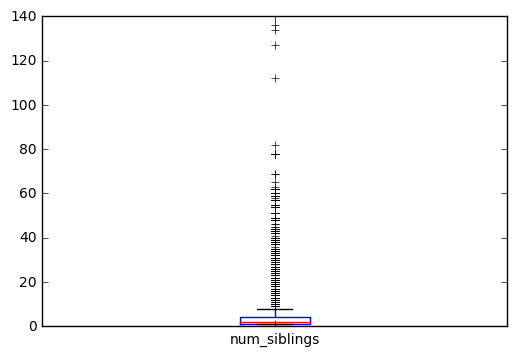
\includegraphics[width=.8\linewidth]{figures06/boxplot_num_siblings}
  \caption{Outliers of \textit{num\_siblings} feature}
\end{subfigure}%
\begin{subfigure}{.5\textwidth}
  \centering
  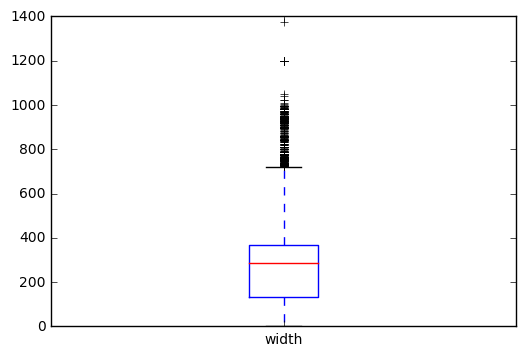
\includegraphics[width=.8\linewidth]{figures06/boxplot_width}
  \caption{Outliers of \textit{width} CSS property}
\end{subfigure}
\caption{Examples of outliers}
\label{fig:outlier}
\end{figure}

\begin{table}[h]
\begin{center}
{\renewcommand{\arraystretch}{1.5}
\begin{tabular}{| p{5cm} | p{5cm}|}
\hline
\textbf{Feature name}	& \textbf{Number of outliers}\\
\hline
num\_siblings	& 476\\
\hline
x\_coords	& 585\\
\hline
y\_coords	& 680\\
\hline
block\_height	& 837\\
\hline
block\_width	& 124\\
\hline
\end{tabular}}
\caption{Number of outliers for several features}
\label{table:outlier}
\end{center}
\end{table}

